\documentclass[usepdftitle=false]{beamer}

\usepackage[T1]{fontenc}

\usepackage[utf8x]{inputenc}
\usepackage{default}
\usepackage{lmodern}
\usepackage{booktabs}

\usepackage{ragged2e} % Kommando\justifying ermöglicht  Blocksatz in Präsentationen
\usepackage{listings}

\mode<presentation>
{\usecolortheme{seahorse,rose}
	\useinnertheme[shadow]{rounded}
	%  \useoutertheme[hideothersubsections,right,width=4em,frame number]{sidebar}
	%  \useoutertheme{infolines}
	%\useoutertheme{split}
	\useoutertheme[subsection=false,footline=authortitle]{miniframes}
	\setbeamercovered{transparent}
}

%seitenzahl in linker ecke
\addtobeamertemplate{navigation symbols}{{\usebeamercolor{section
			in toc}\footnotesize
		\insertframenumber/\inserttotalframenumber}\hspace{48em}}{}
\usepackage{setspace} %mit spacing-Umgebung Zeilenabstand regeln



%%Sprachunterstuetzung
%Englische Silbentrennung, etc.
\usepackage[spanish]{babel}
%Mehrsprachige Literaturliste
\usepackage{babelbib}
%%Graphiken und Farbe
%Graphiken
\usepackage{graphicx} 
%von beamer.cls geladen
%Farbe
\usepackage{color,pgf}
%von beamer.cls geladen
%PDF-Seiten einbinden
\usepackage{pdfpages}
\usepackage{subscript}
\newcommand{\sub}[1]{\textsubscript{#1}}
\newcommand{\Sup}[1]{\textsuperscript{#1}}
\newcommand{\COO}{CO\textsubscript{2}}
\newcommand{\masl}{m~a.s.l.}
\newcommand{\gc}{$^{\circ}$C}
\newcommand{\tilt}{$\sim$}
\newcommand{\blue}[1]{{\color{blue!50!black}#1}}
\newcommand{\Blue}[1]{{\color{blue!50!black}\textbf{#1}}}
\newcommand{\eg}{e.\,g.}
\newcommand{\Eg}{E.\,g.}

% new environment for slides with changes margins
\newenvironment{changemargin}[2]{%
	\begin{list}{}{%
			\setlength{\topsep}{0pt}%
			\setlength{\leftmargin}{#1}%
			\setlength{\rightmargin}{#2}%
			\setlength{\listparindent}{\parindent}%
			\setlength{\itemindent}{\parindent}%
			\setlength{\parsep}{\parskip}%
		}%
		\item[]}{\end{list}}





\hypersetup{
	pdfauthor={Roman Link},
	pdftitle={Estimación de parámetros},
}

%Titelseite
\title{Estimación de los parámetros de la curva de vulnerabilidad}
\subtitle{\normalfont Curso de laboratorio \textit{Mediciones de hidráulica de plantas con el XylEm Plus y la bomba de Scholander}}
\author[R. Link]{Roman Link}
\date{27 de noviembre de 2017}
\institute[University of Göttingen]{
	Department of Plant Ecology and Ecosystem Research\\ Georg August University of Göttingen}
%\titlegraphic{ \vspace*{2em}
%
\includegraphics[width=0.7\textwidth]{logouni.png}}%oder was sch\"oneres

\logo{
\includegraphics[width=20em]{logounisolow.png}}

\usepackage{amsmath,amsfonts,amssymb,pgf}
\usepackage { eulervm }

%\usepackage[round]{natbib}
%\def\newblock{} % hilft gegen absurde fehler mit natbib

\newcommand{\rar}{$\rightarrow$}
\newcommand{\lar}{$\leftarrow$}
\newcommand{\Rar}{$\Rightarrow$}
\newcommand{\Lar}{$\Leftarrow$}
\newcommand{\quelle}[1]{\baselineskip8pt{\tiny \color{gray} #1}}

\newcommand{\tw}{\textwidth}
\newcommand{\ddx}[2]{\frac{\mathrm{d}}{\mathrm{d}#2}#1 }
\newcommand{\ddxx}[2]{\frac{\mathrm{d^2}}{\mathrm{d}#2^2}#1}



\newcommand{\code}[1]{{\footnotesize \color{blue}
		\texttt{#1}}\normalsize\color{black}}


% \input{cc_beamer}
\setbeamerfont{section in toc}{size=\normalsize,series=\bfseries}
\setbeamerfont{title}{series=\bfseries}
\setbeamerfont{frametitle}{size=\Large,series=\bfseries}

\begin{document}
	
	
%%%%%%%%%%%%%%%%%		Title Page			%%%%%%%%%%%%%%%%%%%%%%
\begin{frame}
	\titlepage
\end{frame}

\begin{frame}
	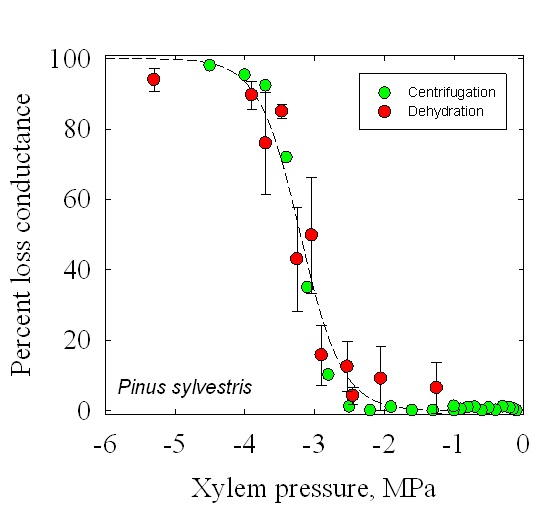
\includegraphics[width = 0.8\tw]{pictures/VC.jpg}\\
	\centering{\quelle{\textbf{Ilustración:}   http://prometheuswiki.org}}
\end{frame}
	
	
\begin{frame}
\frametitle{¿Cuál es la mejor forma de estimar P50?}
\begin{itemize}
  \item Diferentes \Blue{modelos mecanísticos} para la forma de la curva
  \begin{itemize}
	\item Modelo logístico 
	\item Función de sobrevivencia de la distribución de Weibull
    \item \dots 
  \end{itemize}
  \item<2-> Diferentes \Blue{métodos de estimación}
  \begin{itemize}
    \item Linearización
	\item Regresión no linear
	\item \dots
  \end{itemize}
  \item<3-> Diferentes \Blue{programas estadísticas}
  \begin{itemize}
    \item Excel
	\item SAS
	\item R
	\item \dots
  \end{itemize}	
  \item<visible@4| alert@4> Selección de método depende de las circumstancias del experimento, habilidades estadísticas y gusto personal	
\end{itemize}		
\end{frame}

\begin{frame}
\frametitle{Modelo lógistico}
\centering
\begin{equation*}
PLC = \frac{100}{(1 + \mathrm{exp}(S\cdot(\Psi - P50)))}
\end{equation*}
\begin{description}
  \item[PLC] Porcentaje de perdida de conductancia
  \item[$\Psi$] Potencial hídrico
  \item[S]   pendiente (slope)
  \item[P50] Potencial hídrico relacionado a un PLC de 50\% 
\end{description}
\begin{itemize}
	\item<2-> Forma sigmoidal simétrica de la curva
	\item<3-> Asunción implícita: Intercepto de \textbf{y} puede ser mayor de cero   
\end{itemize}
\end{frame}

	
\begin{frame}
\frametitle{Modelo lógistico}
\centering
\only<1>{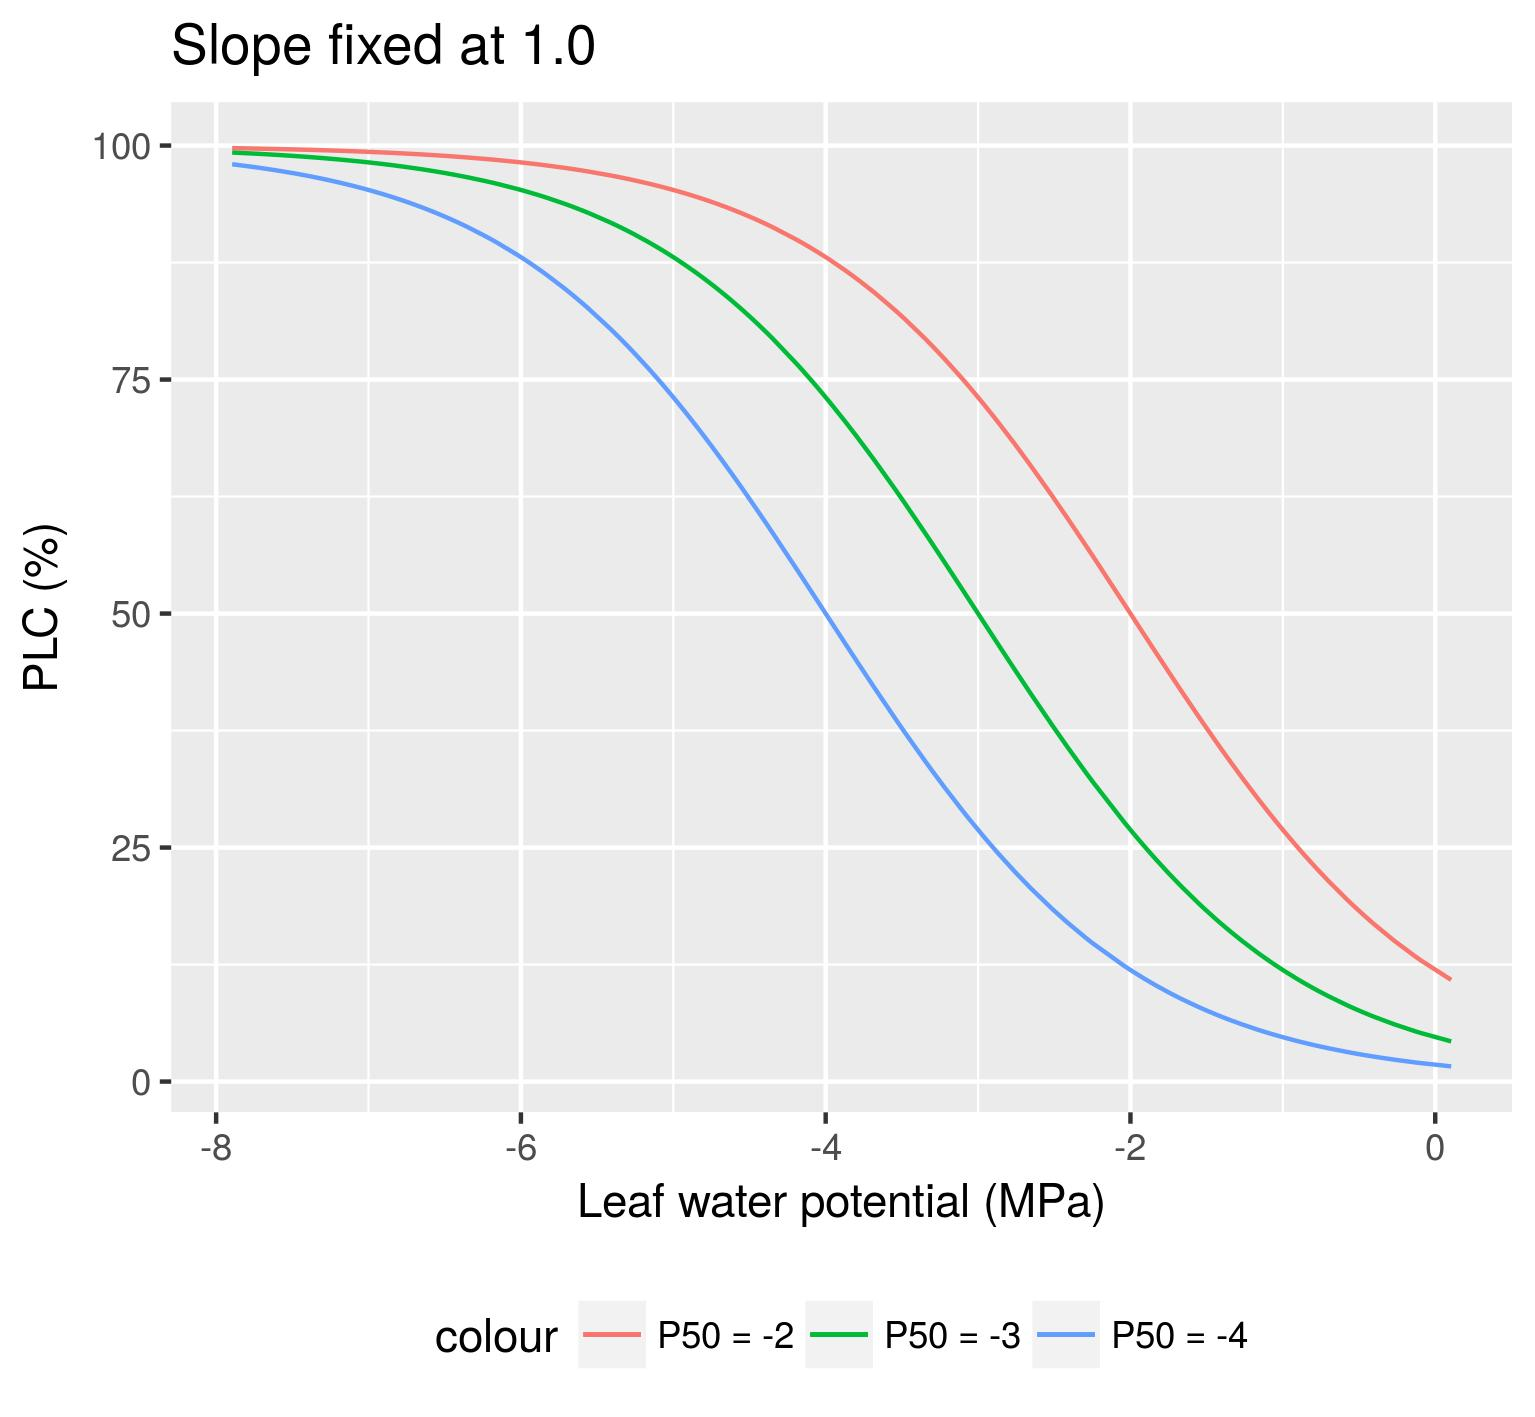
\includegraphics[width = 0.8\tw]{pictures/log_diffp50.jpg}}
\only<2>{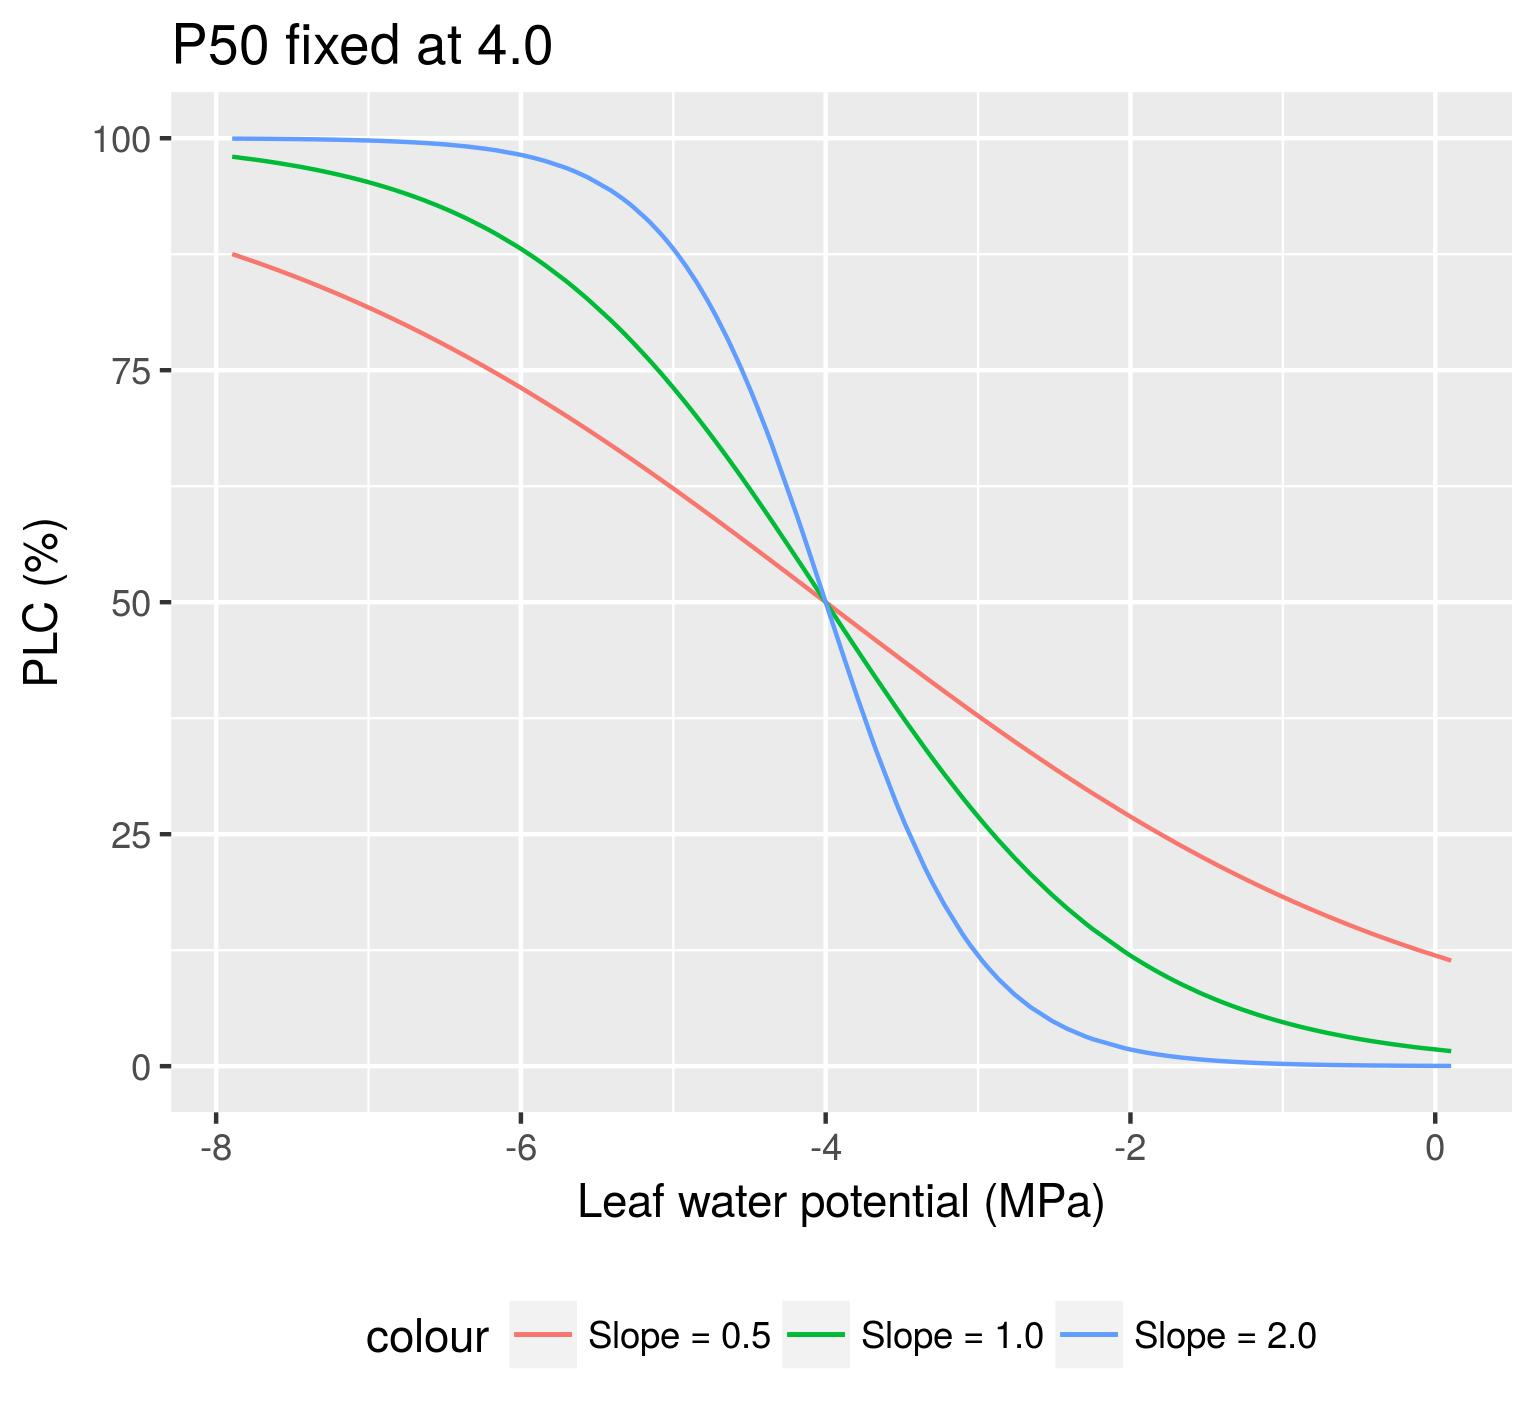
\includegraphics[width = 0.8\tw]{pictures/log_diffslope.jpg}}
\end{frame}

\begin{frame}
\frametitle{Modelo lógistico}
\begin{itemize}
\item<1-> \Blue{Ventajas:}
\begin{itemize}
	\item Puede reflectar "native embolism" -- embolías presentes incluso si la planta esta saturada completamente con agua (debido a eventos de sequía anteriores)
   \item Parámetros con una interpretación mecanística directa
\end{itemize}
\item<2> \Blue{Desventajas:}	
\begin{itemize}
  \item Poco flexible
  \item Solo permite forma sigmoidal
   \item Puede fallar en casos con una subida rápida de PLC en presiones bajas
\end{itemize}
\end{itemize}	
\end{frame}
	



\begin{frame}
\frametitle{Modelo de Weibull}
\begin{equation*}
PLC = 100\cdot (1-exp(-( -\Psi/\lambda)^c))
\end{equation*}
\begin{description}
  \item[PLC] Porcentaje de perdida de conductancia
  \item[$\Psi$] Potencial hídrico
  \item[$\lambda$]  "{}scale parameter"\
  \item[c] "{}shape parameter"\
\end{description}
		\begin{itemize}
            \item<2-> Función de distribución de la distribución de Weibull
			\item<3-> Curva puede ser sigmoidal o tener una forma de "{}r"\ dependiendo del parámetro \texttt{shape}
			\item<4->  Asunción implícita: Intercepto de \textbf{y} restringido a cero
			\end{itemize}	
	\end{frame}	


\begin{frame}
\frametitle{Modelo de Weibull}
\centering
\only<1>{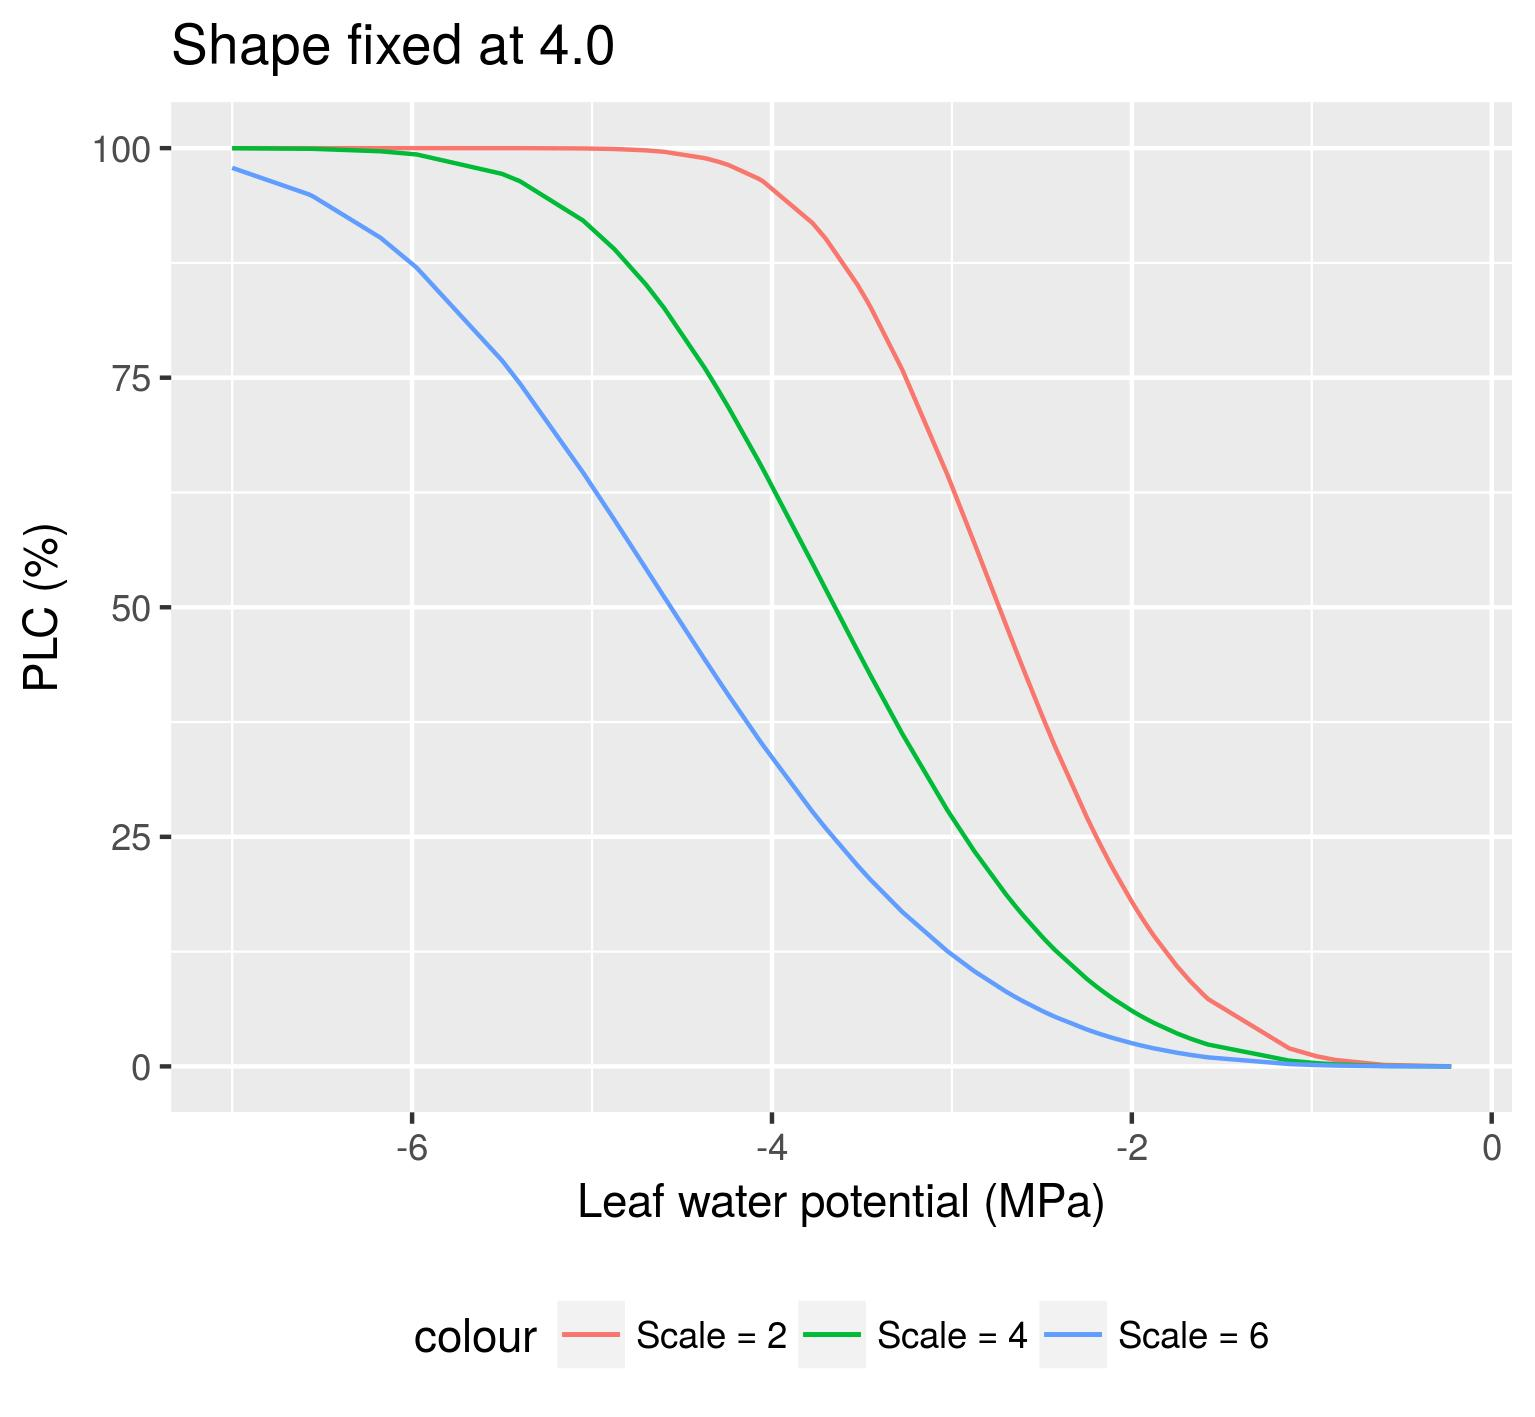
\includegraphics[width = 0.8\tw]{pictures/weib_diffscale.jpg}}
\only<2>{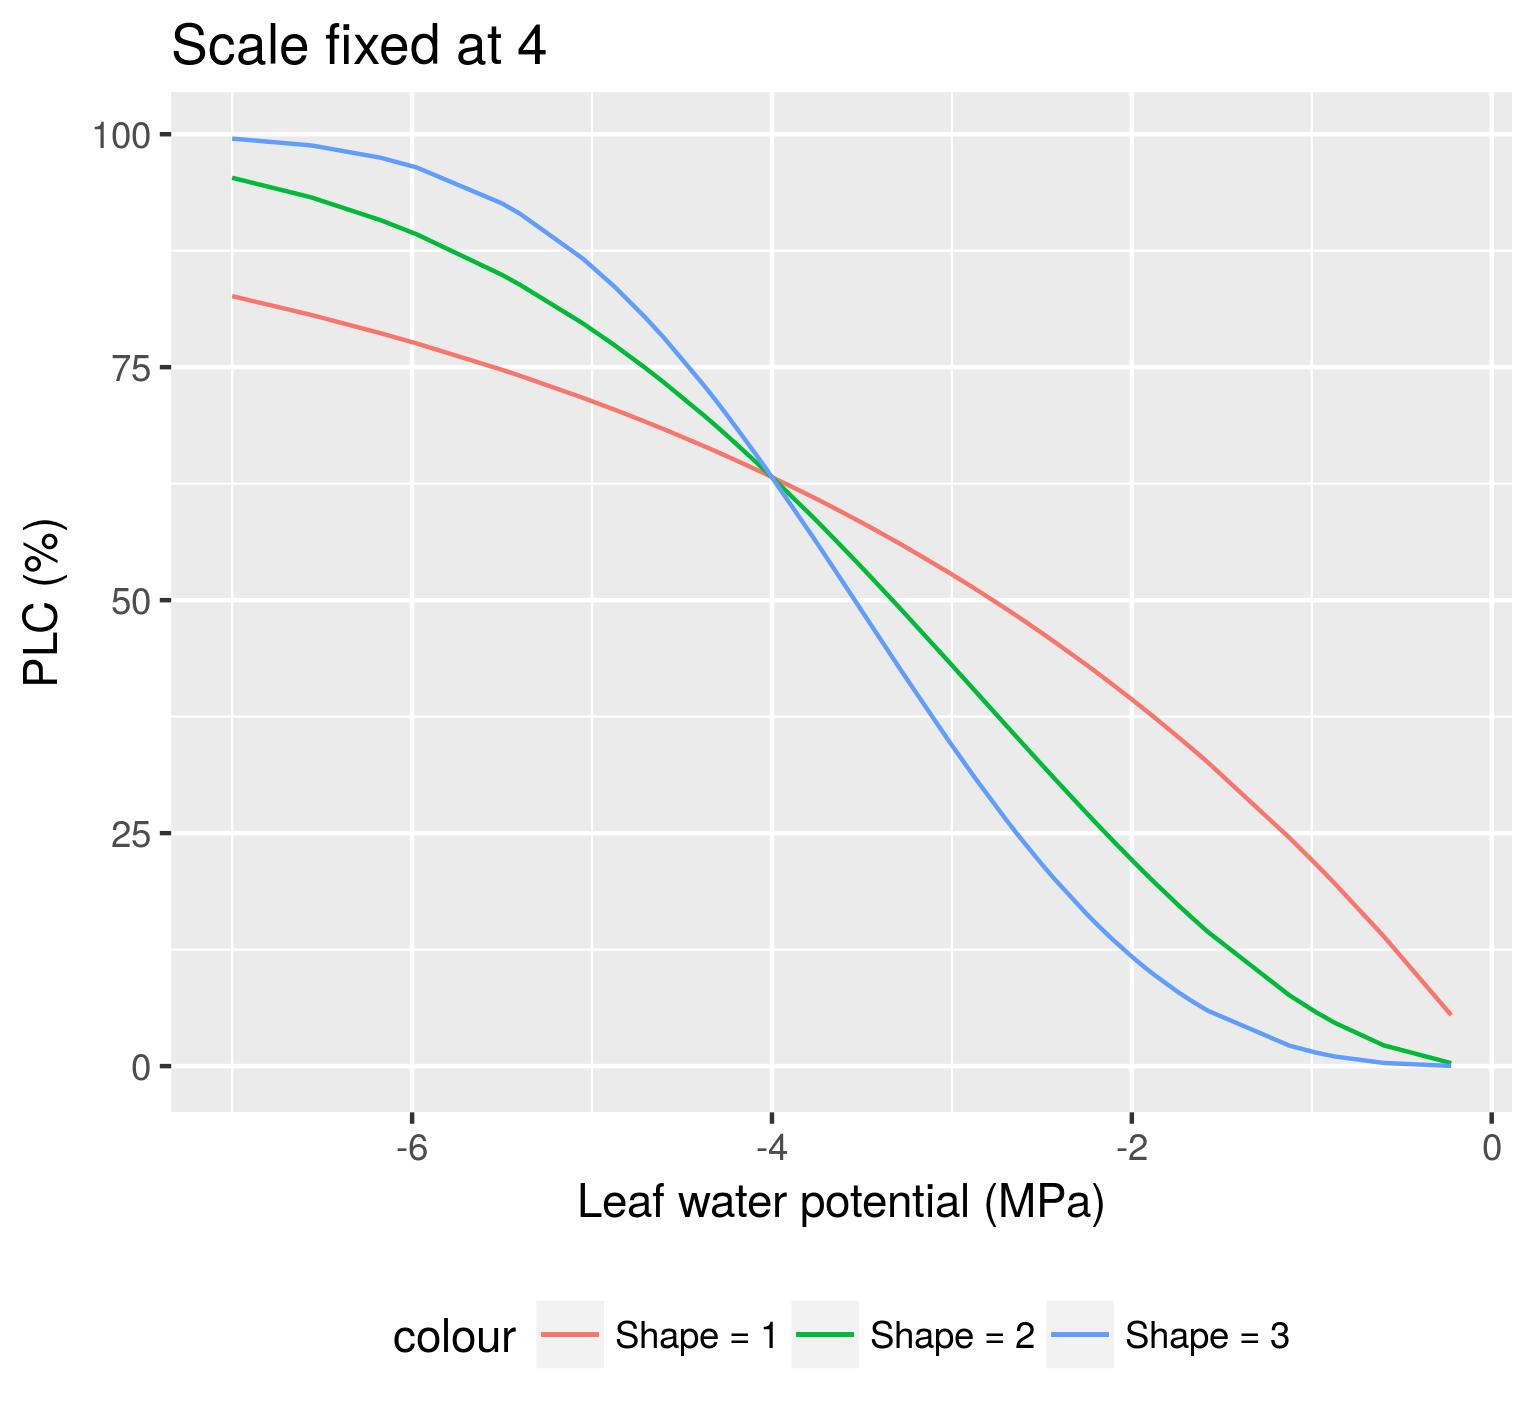
\includegraphics[width = 0.8\tw]{pictures/weib_diffshape.jpg}}
\end{frame}	


\begin{frame}
\frametitle{Modelo de Weibull}
		\begin{itemize}
				\item<1-> \Blue{Ventajas:}
			\begin{itemize}
				\item Muy flexible
				\item Puede acomodar formas sigmoidales y de "{}r"
			\end{itemize}
			\item<2> \Blue{Desventajas:}	
			\begin{itemize}
				\item No permite "native embolism"
				\item Parámetros poco interpretables (PERO: reparameterización con P50 es posible)
			\end{itemize}
		\end{itemize}	
	\end{frame}	


\begin{frame}
\frametitle{Interpretación como función de distribución}
\centering
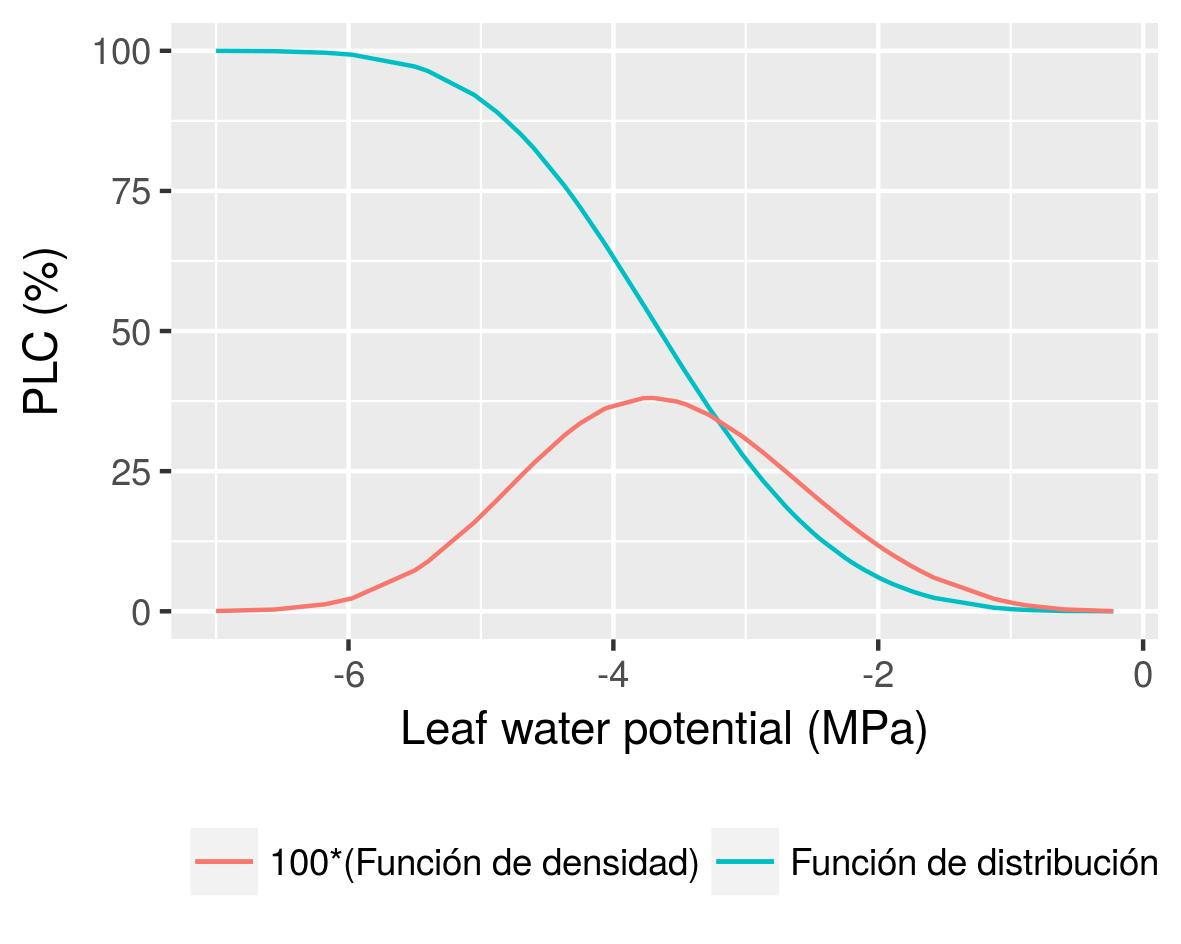
\includegraphics[width = 0.6\tw]{pictures/weib_pdf.jpg}
\begin{itemize}
   \item<only@1> Si se interpreta la curva de vulnerabilidad como una función de distribución (distribución de Weibull/distribución logística)\dots
   \item<only@2>\dots se puede interpretar la función de densidad correspondiente como la función de densidad de la distribución de los potenciales en las cuales se están embolizando los vasos
\end{itemize}
\end{frame}	
	
	
	\begin{frame}
		\frametitle{Problemas con la estimación de parámetros}
		\begin{itemize}
			\item<1-> Datos de curvas de vulnerabilidad casi siempre tienen una \alert<1>{forma jerárquica}
			\begin{itemize}
				\item Varios árboles por especies
				\item Varias submuestras por árbol
				\item Varias mediciones por submuestra
			\end{itemize}
			\item<2-> No se necesita estimados precisos de los parámetros de {\alert<2>{árbol especifico}}, si no un estimado de los parametrós de un {\alert<2>{árbol promedio}} de una especie y de la variabilidad interespecífica de los parámetros
			\item<3-> Si se usa los parámetros estimados de curvas de vulnerabilidad como variable de respuesta en otros modelos, se tiene que tener en cuenta el \alert<3>{incertidumbre de los estimados}
			\item<visible@4| alert@4>[\Rar] Solución para todos estos problemas: \textbf{Modelos jerárquicos ("modelos mixtos")}
		\end{itemize}	
	\end{frame}	
		
\begin{frame}
\frametitle{Ejemplo de un modelo jerárquico para curvas de vulnerabilidad}
\begin{itemize}
\item<1-> Datos de Pierre-André Waite (Universidad de Göttingen) 

\item<2-> 2 parcelas de plantaciones de palma de aceite en Indonesia
\begin{itemize}
\item 12 árboles
\item 2--3 mediciones por árbol
\end{itemize}
\item<3> Ejemplo de modelo usando R con el paquete \texttt{nlme} 
\end{itemize} 

\end{frame}	

\begin{frame}[fragile]
\begin{lstlisting}
> # Estructura de datos
>
> data1 
# A tibble: 34 x 4
        PLC    psi   plot      palm
      <dbl>  <dbl> <fctr>    <fctr>
 1 93.31132 -7.000    HO1 HO1_01694
 2 89.51220 -6.550    HO1 HO1_01697
 3 76.41509 -5.500    HO1 HO1_01674
 4 94.29929 -4.875    HO1 HO1_01676
 5 34.73684 -4.600    HO1 HO1_01680
 6 47.50403 -4.375    HO1 HO1_01676
 7 21.29032 -4.240    HO1 HO1_01676
 8 47.08904 -3.450    HO1 HO1_01697
 9 97.91216 -3.275    HO1 HO1_01697
10 84.31772 -2.875    HO1 HO1_01694
# ... with 24 more rows
\end{lstlisting}
\end{frame}		

\begin{frame}[fragile]
\footnotesize
\begin{lstlisting}
> # modelo no-lineal mixto
>
> require(nlme)
> mod2 <- nlme(PLC ~ 100/(1 + exp(slope*(psi - p50))),
+              fixed  = slope + p50 ~ plot,
+              random = slope + p50 ~ 1|palm,
+              data = data1,
+              start = c(slope = 1, 0, p50 = -2, 0), 
+              method = "ML",
+              control = nlmeControl(maxiter = 1000, 
+                                    pnlsMaxIter = 1000, 
+                                    msMaxIter = 1000,
+                                    niterEM = 100))
\end{lstlisting}
\end{frame}	

\begin{frame}[fragile, allowframebreaks]
\footnotesize
\begin{lstlisting}
> # > resultados del modelo             
> summary(mod2)
Nonlinear mixed-effects model fit by maximum likelihood
  Model: PLC ~ 100/(1 + exp(slope * (psi - p50))) 
 Data: data1 
       AIC      BIC    logLik
  325.2443 337.4552 -154.6222

Random effects:
 Formula: list(slope ~ 1, p50 ~ 1)
 Level: palm
 Structure: General positive-definite, Log-Cholesky param...
                  StdDev       Corr  
slope.(Intercept) 1.795721e-04 sl.(I)
p50.(Intercept)   2.039200e-05 0     
Residual          2.284592e+01       




Fixed effects: slope + p50 ~ plot 
                      Value Std.Error DF   t-value p-value
slope.(Intercept)  0.567227 0.2156021 19  2.630897  0.0165
slope.plotHO3      0.827329 0.6499720 19  1.272869  0.2184
p50.(Intercept)   -3.422122 0.4913243 19 -6.965098  0.0000
p50.plotHO3        1.534501 0.5443090 19  2.819173  0.0110
 Correlation: 
                sl.(I) sl.HO3 p50.(I
slope.plotHO3   -0.332              
p50.(Intercept)  0.055 -0.018       
p50.plotHO3     -0.050 -0.124 -0.903

Standardized Within-Group Residuals:
       Min         Q1        Med         Q3        Max 
-1.7554167 -0.7472870 -0.1248341  0.3211212  2.1884542 

Number of Observations: 34
Number of Groups: 12
\end{lstlisting}
\end{frame}	

\begin{frame}
\frametitle{Plot of modeling results}
\only<1>{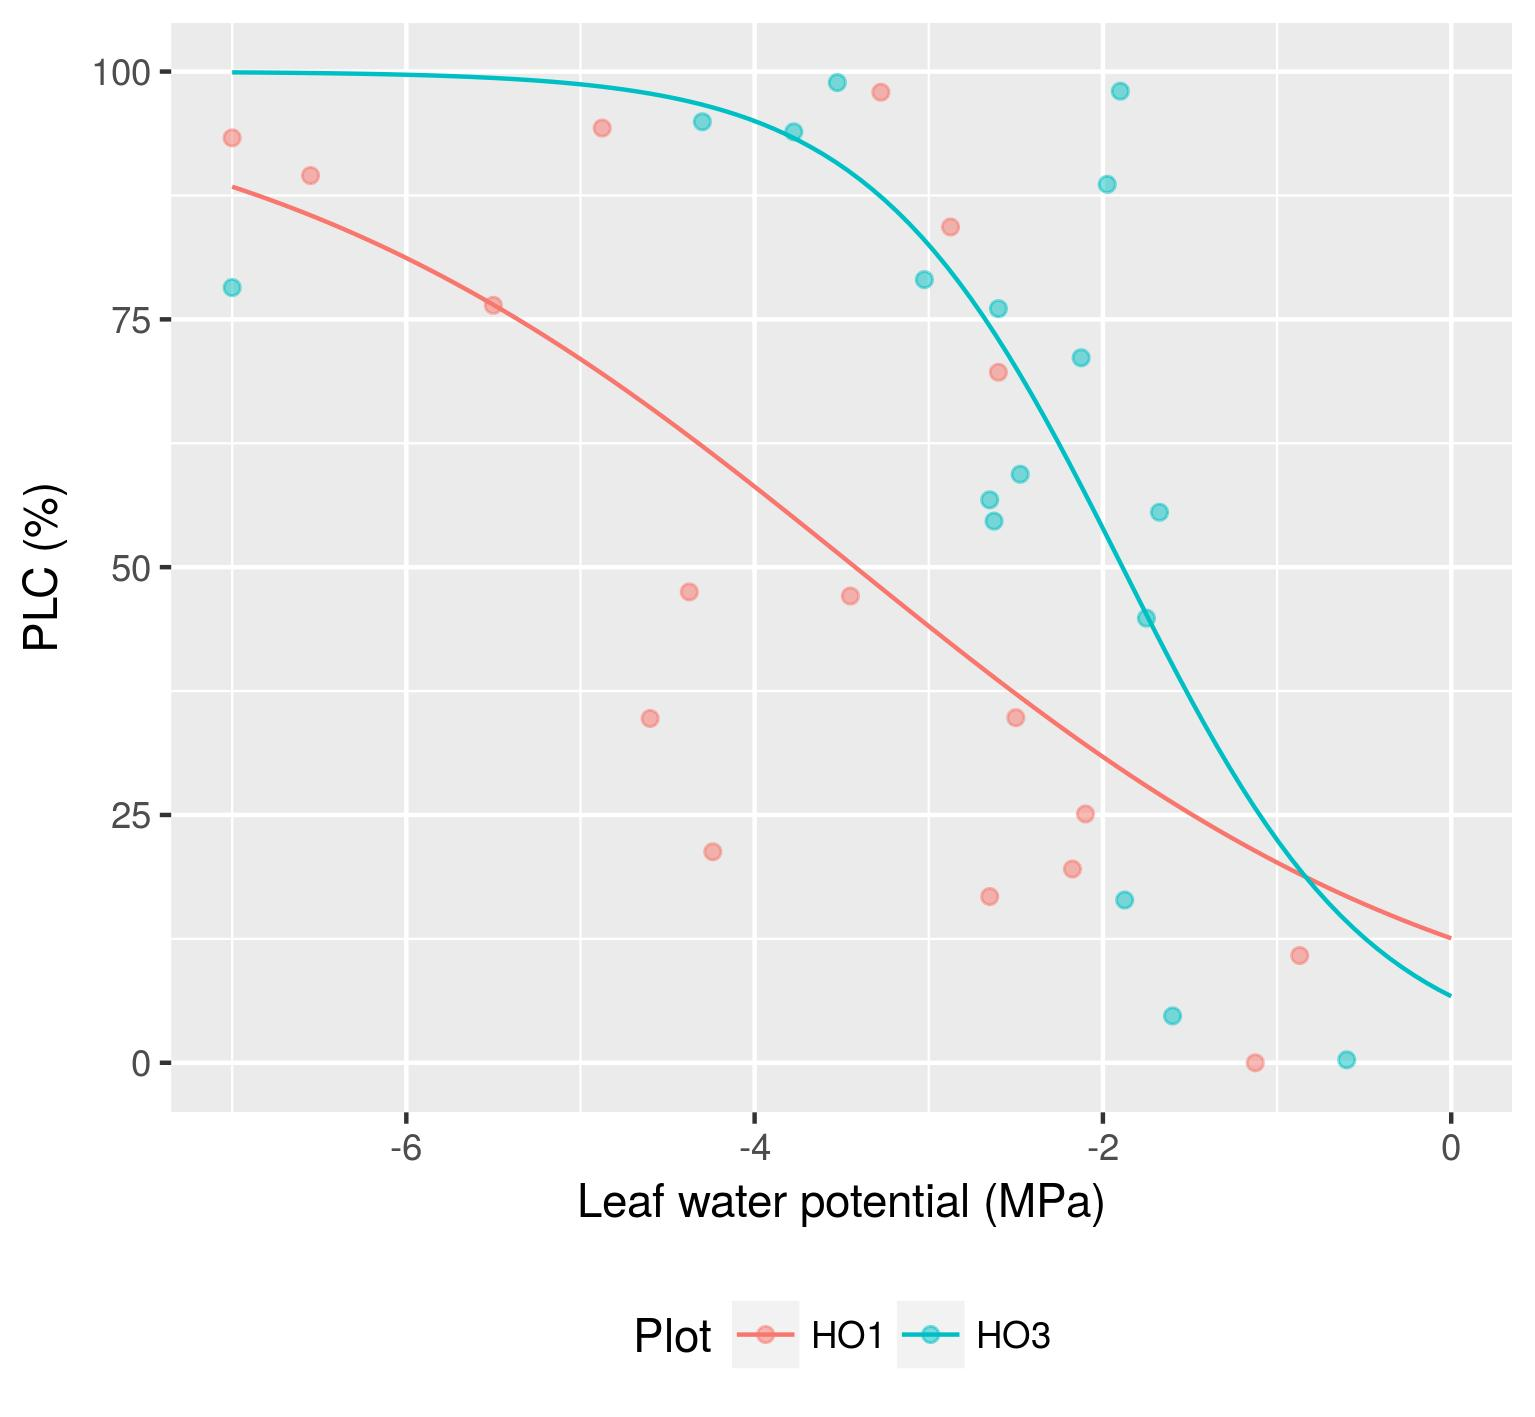
\includegraphics[width = 0.8\tw]{pictures/VC_pierre_pres.jpg}}
\only<2>{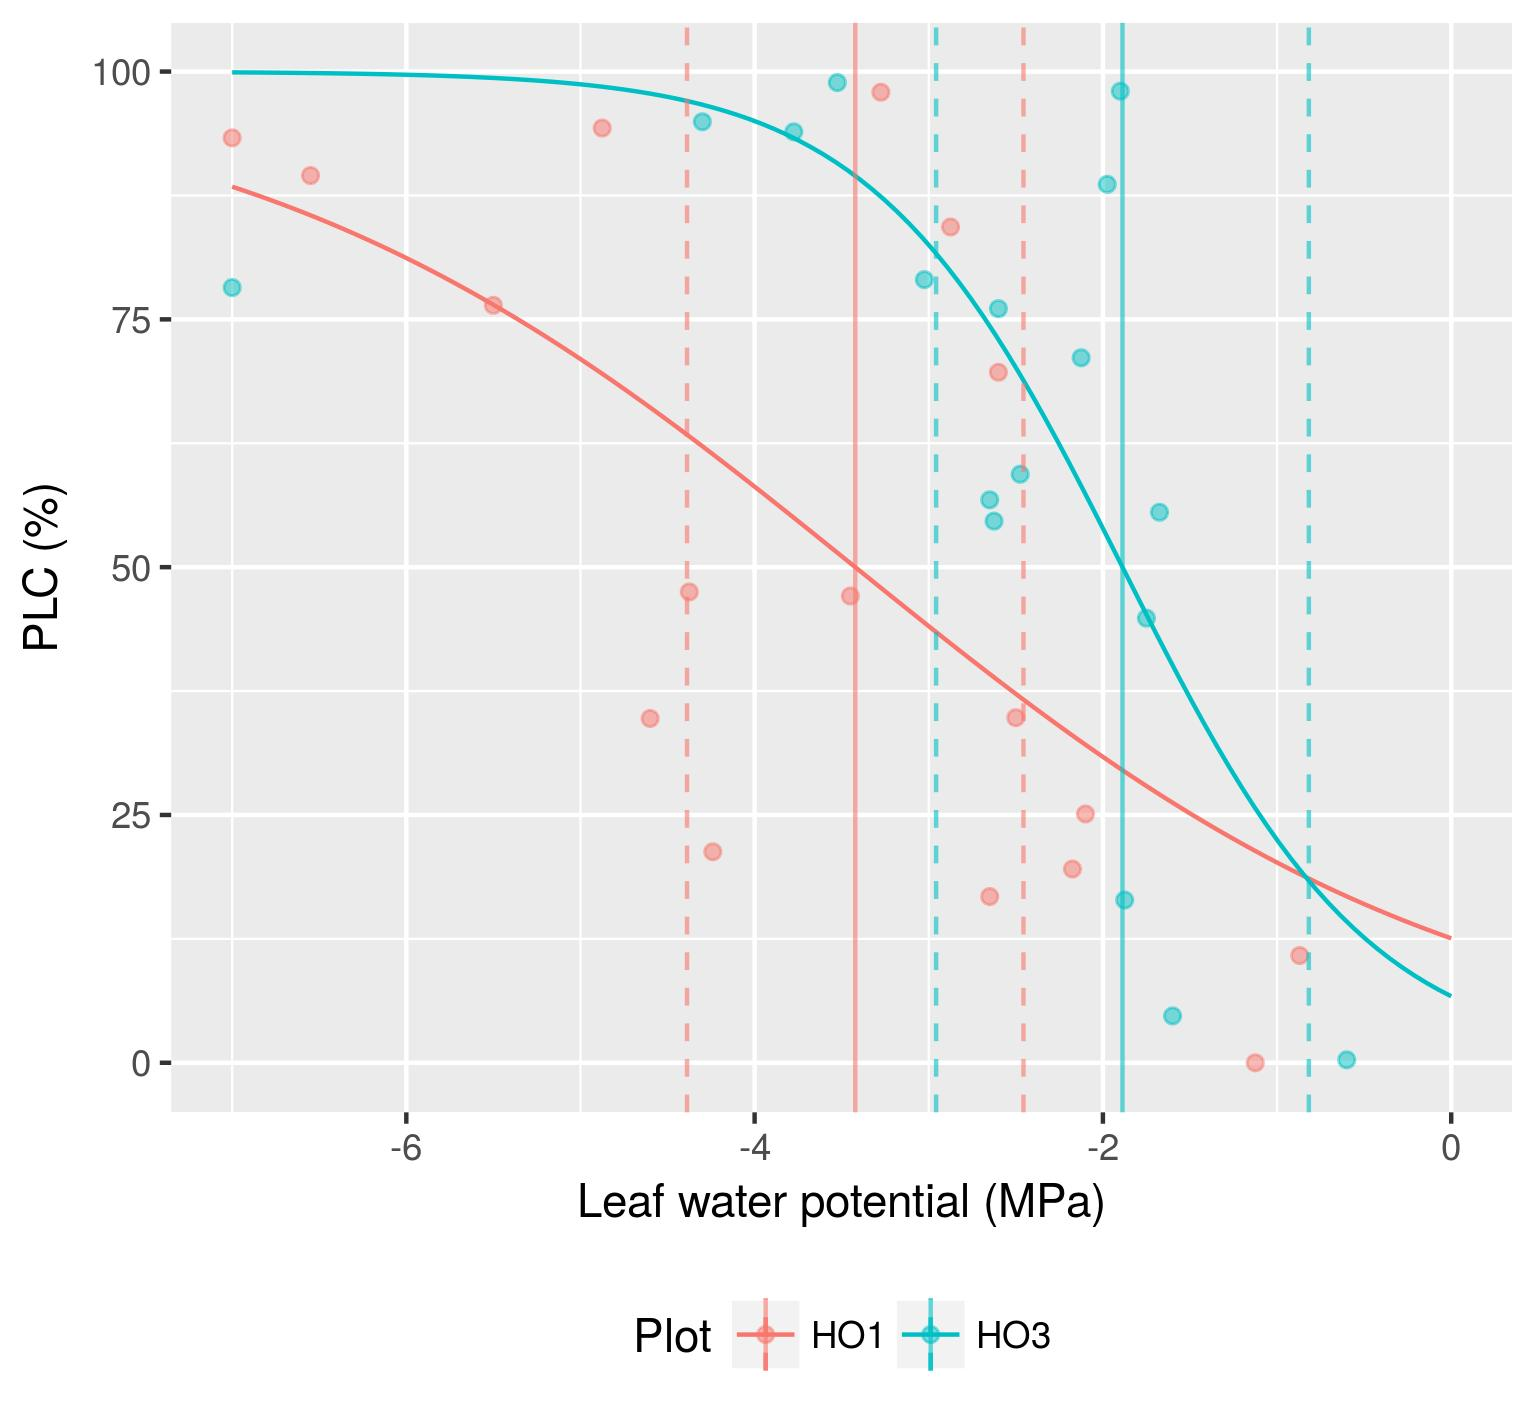
\includegraphics[width = 0.8\tw]{pictures/VC_pierre_pres1.jpg}}
\end{frame}
\end{document}
